\documentclass{article}

\usepackage{fancyhdr}
\usepackage{extramarks}
\usepackage{amsmath}
\usepackage{amsthm}
\usepackage{amsfonts}
\usepackage{tikz}
\usepackage{tikz-qtree}
\usepackage[plain]{algorithm}
\usepackage{algpseudocode}
\usepackage{listings}
\usepackage{enumerate}
\lstset{breaklines=true}

\usetikzlibrary{automata,positioning,calc}

%
% Basic Document Settings
%

\topmargin=-0.45in
\evensidemargin=0in
\oddsidemargin=0in
\textwidth=6.5in
\textheight=9.0in
\headsep=0.25in

\linespread{1.1}

\pagestyle{fancy}
\lhead{\hmwkAuthorName}
\chead{\hmwkClass\ (\hmwkClassInstructor): \hmwkTitle}
\rhead{\firstxmark}
\lfoot{\lastxmark}
\cfoot{\thepage}

\renewcommand\headrulewidth{0.4pt}
\renewcommand\footrulewidth{0.4pt}

\setlength\parindent{0pt}

%
% Create Problem Sections
%

\newcommand{\enterProblemHeader}[1]{
    \nobreak\extramarks{}{Problem \arabic{#1} continued on next page\ldots}\nobreak{}
    \nobreak\extramarks{Problem \arabic{#1} (continued)}{Problem \arabic{#1} continued on next page\ldots}\nobreak{}
}

\newcommand{\exitProblemHeader}[1]{
    \nobreak\extramarks{Problem \arabic{#1} (continued)}{Problem \arabic{#1} continued on next page\ldots}\nobreak{}
    \stepcounter{#1}
    \nobreak\extramarks{Problem \arabic{#1}}{}\nobreak{}
}

\newcommand{\bipgraph}[2]{%
    \begin{tikzpicture}[every node/.style={circle,draw}]
    \foreach \xitem in {1,...,#1}
    {%
    % first set
    \node at (0,\xitem) (a\xitem) {};
    % second set
    \node at (2,\xitem) (b\xitem) {};   
    }%

    % connections
    \foreach \x [count=\xi] in {#2}
    {% 
    \foreach \tritem in \x % <-- Here no braces to make it a foreach list also not \xi but \x
    \draw(a\xi) -- (b\tritem);
    }
    \end{tikzpicture}  
}

\newcommand{\bipgraphComplete}[1]{%
    \begin{tikzpicture}[every node/.style={circle,draw}]
    \foreach \xitem in {1,...,#1}
    {%
    % first set
    \node at (0,\xitem) (a\xitem) {};
    % second set
    \node at (2,\xitem) (b\xitem) {};   
    }%

    % connections
    \foreach \x in {1,...,#1}
    {% 
    \foreach \y in {1,...,#1}
        \draw(a\x) -- (b\y);
    }
    \end{tikzpicture}  
}

\setcounter{secnumdepth}{0}
\newcounter{partCounter}
\newcounter{homeworkProblemCounter}
\setcounter{homeworkProblemCounter}{1}
\nobreak\extramarks{Problem \arabic{homeworkProblemCounter}}{}\nobreak{}

%
% Homework Problem Environment
%
% This environment takes an optional argument. When given, it will adjust the
% problem counter. This is useful for when the problems given for your
% assignment aren't sequential. See the last 3 problems of this template for an
% example.
%
\newenvironment{homeworkProblem}[1][-1]{
    \ifnum#1>0
        \setcounter{homeworkProblemCounter}{#1}
    \fi
    \section{Problem \arabic{homeworkProblemCounter}}
    \setcounter{partCounter}{1}
    \enterProblemHeader{homeworkProblemCounter}
}{
    \exitProblemHeader{homeworkProblemCounter}
}

%
% Homework Details
%   - Title
%   - Due date
%   - Class
%   - Section/Time
%   - Instructor
%   - Author
%

\newcommand{\hmwkTitle}{Homework\ \#11}
\newcommand{\hmwkDueDate}{March 11, 2015}
\newcommand{\hmwkClass}{Graph Theory}
\newcommand{\hmwkClassTime}{MWF 9:15}
\newcommand{\hmwkClassInstructor}{Professor McGinley}
\newcommand{\hmwkAuthorName}{Rick Sullivan}

%
% Title Page
%

\title{
    \vspace{2in}
    \textmd{\textbf{\hmwkClass:\ \hmwkTitle}}\\
    \normalsize\vspace{0.1in}\small{Due\ on\ \hmwkDueDate}\\
    \vspace{0.1in}\large{\textit{\hmwkClassInstructor\ \hmwkClassTime}}
    \vspace{3in}
}

\author{\textbf{\hmwkAuthorName}}
\date{}

\renewcommand{\part}[1]{\textbf{\large Part \Alph{partCounter}}\stepcounter{partCounter}\\}

%
% Various Helper Commands
%

% Useful for algorithms
\newcommand{\alg}[1]{\textsc{\bfseries \footnotesize #1}}

% For derivatives
\newcommand{\deriv}[1]{\frac{\mathrm{d}}{\mathrm{d}x} (#1)}

% For partial derivatives
\newcommand{\pderiv}[2]{\frac{\partial}{\partial #1} (#2)}

% Integral dx
\newcommand{\dx}{\mathrm{d}x}

% Alias for the Solution section header
\newcommand{\solution}{\textbf{\large Solution}}

% Probability commands: Expectation, Variance, Covariance, Bias
\newcommand{\E}{\mathrm{E}}
\newcommand{\Var}{\mathrm{Var}}
\newcommand{\Cov}{\mathrm{Cov}}
\newcommand{\Bias}{\mathrm{Bias}}

\begin{document}

\maketitle

\pagebreak

\begin{homeworkProblem}
    Compute \(\chi_1(G)\) for the graph below.
    \\
    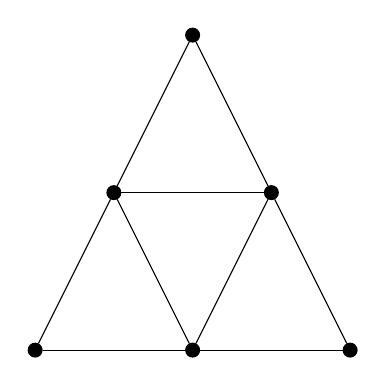
\begin{tikzpicture}[vertex/.style={circle,draw,fill=black,inner sep=0pt,minimum size=5pt}]
        \node[vertex] at (2, 4) (a) {};
        \node[vertex] at (1, 2) (b) {};
        \node[vertex] at (3, 2) (c) {};
        \node[vertex] at (0, 0) (d) {};
        \node[vertex] at (2, 0) (e) {};
        \node[vertex] at (4, 0) (f) {};

        \draw(a) -- (b);
        \draw(a) -- (c);
        \draw(b) -- (c);
        \draw(b) -- (d);
        \draw(b) -- (e);
        \draw(c) -- (e);
        \draw(c) -- (f);
        \draw(d) -- (e);
        \draw(e) -- (f);
    \end{tikzpicture}
    \\

    \textbf{Solution}
    \\

    \begin{proof}
        \(\Delta(G)=4\), so \(\chi(G)\) will be either 4 or 5. If it is 4, \(G\) has a 1-factorization. Assume \(\chi(G)=4\) and consider one of the edges on the inner triagular cycle in \(G\). This must be placed into a perfect matching. Both end vertices on this edge are the only two neighbors of one of the corner vertices in \(G\). Therefore, this vertex cannot be placed into a perfect matching if this edge is part of the matching. This means that \(\chi(G)!=4\), so \(\chi(G)=5\).
    \end{proof}
\end{homeworkProblem}

\begin{homeworkProblem}
    Compute the chromatic polynomials for the graphs below.
    \\

    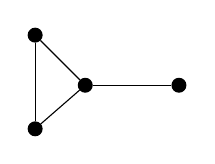
\begin{tikzpicture}[vertex/.style={circle,draw,fill=black,inner sep=0pt,minimum size=5pt}]
        \node[vertex] (a) {};
        \node[vertex] (b) [below=1cm of a] {};
        \node[vertex] (c) [below right=0.71cm of a] {};
        \node[vertex] (d) [right=1cm of c] {};

        \draw(a) -- (b);
        \draw(a) -- (c);
        \draw(b) -- (c);
        \draw(c) -- (d);
    \end{tikzpicture}
    \hspace{0.5in}
    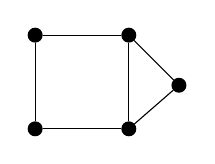
\begin{tikzpicture}[vertex/.style={circle,draw,fill=black,inner sep=0pt,minimum size=5pt}]
        \node[vertex] (a) {};
        \node[vertex] (b) [below=1cm of a] {};
        \node[vertex] (c) [right=1cm of b] {};
        \node[vertex] (d) [right=1cm of a] {};
        \node[vertex] (e) [below right=0.71cm of d] {};

        \draw(a) -- (b);
        \draw(a) -- (d);
        \draw(b) -- (c);
        \draw(c) -- (d);
        \draw(c) -- (e);
        \draw(d) -- (e);
    \end{tikzpicture}
    \\

    \textbf{Graph a}
    \\

    We have \(k\) choices for the top vertex, with \(k-1\) and then \(k-2\) for the two other vertices in the three-cycle. The final vertex can be any color but the adjacent, so we have \(k-1\) choices. Therefore, the chromatic polynomial is \((k)(k-1)^2(k-2)\).
    \\

    \textbf{Graph b}
    \\

    Starting with coloring the rightmost vertex, we have \(k\) options, followed by \(k-1\) and \(k-2\) colorings for the adjacent vertices, like above. We have two cases for each of the two left-side vertices. If one of them is the color of the opposing vertex in the square-cycle, the remaining vertex has \(k-1\) color options. Otherwise, the remaining vertex will have \(k-2\) possible colorings.
    \\
    Therefore, our chromatic polynomial is 
    \[
        \begin{split}
            &(k)(k-1)(k-2)\left( (k-1) + (k-1)(k-2) \right)
            \\
            &=(k)(k-1)^2(k-2)\left(1 + (k-2) \right)
            \\
            &=(k)(k-1)^3(k-2)
        \end{split}
    \]

\end{homeworkProblem}
\begin{homeworkProblem}
    Prove that \(k^4-4k^3+3k^2\) is not a chromatic polynomial.
    \\

    \textbf{Solution}
    \\

    By the theorem we covered in class, the highest power in \(\chi(G,k)\) gives the order of \(G\), so \(G\) has 4 vertices. The theorem also states that the exponent of the last nonzero term is the number of components of \(G\). Additionally, the coefficient of the second term must be the negative number of edges in \(G\). Therefore, \(G\) has four vertices and four edges in two components. Consider the two cases of components:
    \begin{enumerate}
        \item Both components have 2 vertices. In this case, \(G\) could only have 2 possible edges.
        \item One component has 1 vertex, the other has 3 vertices. 
            The component with 1 vertex has no edges, and a 3 vertex graph cannot have 4 edges. 
    \end{enumerate}

    Neither of these cases are possible, so \(k^4-4k^3+3k^2\) must not be a chromatic polynomial.

\end{homeworkProblem}
\begin{homeworkProblem}
    Prove that the sum of the coefficients of \(\chi (G,k)\) is 0 unless \(G\) has no edges. (Hint: when a function is a polynomial, how can one obtain the sum of the coefficients?)
    \\

    \textbf{Solution}
    \\

    \begin{proof}
    Calculating \(\chi(G,1)\) gives us the sum of the coefficients of the chromatic polynomial.
    Assume \(\chi(G,1)\) is nonzero. Therefore, there exists a vertex coloring of \(G\) with exactly one color. A viable coloring requires that no two same-colored vertices are adjacent, so no vertices are adjacent. Therefore, if \(\chi(G,1)\), the sum of the coefficients of \(\chi(G,k)\), is nonzero, \(G\) has no edges.
    \end{proof}
\end{homeworkProblem}
\pagebreak
\begin{homeworkProblem}
    Without computing them, give a short proof that the chromatic polynomials of the two graphs below are equal.
    \\
    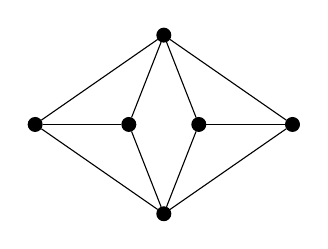
\begin{tikzpicture}[vertex/.style={circle,draw,fill=black,inner sep=0pt,minimum size=5pt}]
        \node[vertex] (a) {};
        \node[vertex] (b) [below left=1cm and 1.5cm of a] {};
        \node[vertex] (c) [right=1cm of b] {};
        \node[vertex] (e) [below right=1cm and 1.5cm of a] {};
        \node[vertex] (d) [left=1cm of e] {};
        \node[vertex] (f) [below right=1cm and 1.5cm of b] {};

        \draw(a) -- (b);
        \draw(a) -- (c);
        \draw(a) -- (d);
        \draw(a) -- (e);
        \draw(b) -- (c);
        \draw(d) -- (e);
        \draw(f) -- (b);
        \draw(f) -- (c);
        \draw(f) -- (d);
        \draw(f) -- (e);
    \end{tikzpicture}
    \hspace{0.5in}
    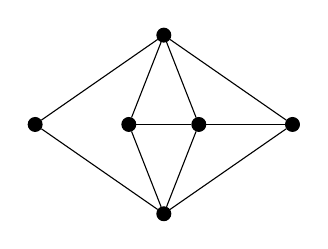
\begin{tikzpicture}[vertex/.style={circle,draw,fill=black,inner sep=0pt,minimum size=5pt}]
        \node[vertex] (a) {};
        \node[vertex] (b) [below left=1cm and 1.5cm of a] {};
        \node[vertex] (c) [right=1cm of b] {};
        \node[vertex] (e) [below right=1cm and 1.5cm of a] {};
        \node[vertex] (d) [left=1cm of e] {};
        \node[vertex] (f) [below right=1cm and 1.5cm of b] {};

        \draw(a) -- (b);
        \draw(a) -- (c);
        \draw(a) -- (d);
        \draw(a) -- (e);
        \draw(c) -- (d);
        \draw(d) -- (e);
        \draw(f) -- (b);
        \draw(f) -- (c);
        \draw(f) -- (d);
        \draw(f) -- (e);
    \end{tikzpicture}
    \\

    \textbf{Solution}
    \\


    \begin{proof}
        By applying a single iteration of the algorithm discussed in class, both of these graphs can be reduced to the difference between the chromatic polynomials of the following two graphs
        \\
        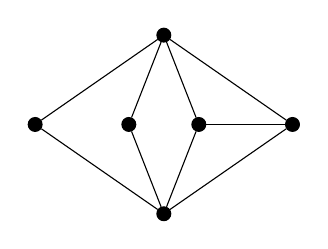
\begin{tikzpicture}[vertex/.style={circle,draw,fill=black,inner sep=0pt,minimum size=5pt}]
            \node[vertex] (a) {};
            \node[vertex] (b) [below left=1cm and 1.5cm of a] {};
            \node[vertex] (c) [right=1cm of b] {};
            \node[vertex] (e) [below right=1cm and 1.5cm of a] {};
            \node[vertex] (d) [left=1cm of e] {};
            \node[vertex] (f) [below right=1cm and 1.5cm of b] {};

            \draw(a) -- (b);
            \draw(a) -- (c);
            \draw(a) -- (d);
            \draw(a) -- (e);
            \draw(d) -- (e);
            \draw(f) -- (b);
            \draw(f) -- (c);
            \draw(f) -- (d);
            \draw(f) -- (e);
        \end{tikzpicture}
        \hspace{0.5in}
        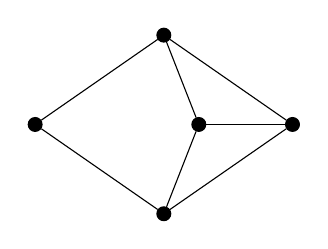
\begin{tikzpicture}[vertex/.style={circle,draw,fill=black,inner sep=0pt,minimum size=5pt}]
            \node[vertex] (a) {};
            \node[vertex] (b) [below left=1cm and 1.5cm of a] {};
            \node[vertex] (e) [below right=1cm and 1.5cm of a] {};
            \node[vertex] (d) [left=1cm of e] {};
            \node[vertex] (f) [below right=1cm and 1.5cm of b] {};

            \draw(a) -- (b);
            \draw(a) -- (d);
            \draw(a) -- (e);
            \draw(d) -- (e);
            \draw(f) -- (b);
            \draw(f) -- (d);
            \draw(f) -- (e);
        \end{tikzpicture}
        \\
        so both graphs have the same chromatic polynomial.
    \end{proof}

\end{homeworkProblem}

\end{document}
